 
\section{Our focus and plan}

% % % TODO % % % %
%from rules: Innovative technology (if any) TODO describe usage of STRANDS
%from rules: Reusability of the system or parts thereof - see STRANDS
This section summarises our intentions for our system this year. We would like to aim for high reusability of the code in our robotic system and to demonstrate that the current state of the art in AI algorithms mixed with our extensions can be successfully used to produce a robust, effective and complete robotic system with domestic applications.  

\subsection{Catering for Granny Annie’s Comfort}


%The problem of speech recognition is often discussed within the robotic community. It is something, which is necessary for future robots to cooperate with humans. Assuming a robot is working at Granny's flat, the robot can learn and adapt to her voice, which will increases its performance over time. Moreover, Granny is living alone, thus, it can be assumed that the level of background noise is minimal. In contrast, during the competition, speech recognition provides a lot of challenges. The background noise is really high during competition because of the spectators. Furthermore, the person playing Granny Annie changes, hence a robot cannot improve its behaviour. We do not plan to develop our system from scratch, rather we plan to use CMU Sphinx - Open Source Toolkit For Speech Recognition \cite{cmu}. 
%Moreover, we might cooperate with a Natural Language Processing group within our school to improve the system's behaviour.

%For a challenge, where the robot approaches humans, we will use the opportunity for closer cooperation with the STRANDS \cite{strands} project, as our robotics group within our school leads this project. Especially, a cooperation with Christian Dondrup, a PhD student at the University of Lincoln, might be beneficial in this stage, as he is working on Human Robot Interaction.

%The second part of this task - bringing someone a specific object - is even more challenging as it includes two large robotics domains, computer vision and manipulation. As our robot has no manipulator this year (see Section \ref{sec:hardware}), we might be able to perform only object search. We might benefit from experiences from a previous project in our robotic group - CogX \cite{cogx}. In this project, one of the robot's abilities was to search for known objects by taking into account common sense knowledge (i.e. prior knowledge) in the form of probabilities of objects' presence in different rooms. However, this will still require a lot of effort from us, as the robot was not using ROS before and we will need to understand and integrate bits into our system. We assume to work on this part next year.

\subsection{Welcoming visitors}

Last year, we successfully completed this task. Hence, the main structure is built. We are improving the uniform detection to increase robustness. 
Moreover, we are improving our human detection system, for example, we are making tests with an IR camera.

\subsection{Getting to know my home}

We proved last year, that our system is able to robustly detect doors using laser rangefinder. Moreover, we were able to detect changes in furniture. However, the robot was unable to detect exact position of the furniture which is important to be able to use the knowledge later. 
Therefore, we would like to integrate one of the STRANDS packages, which is able to detect dynamic clusters from 3D point clouds and recognise to which object they belong. 
%TODO citation
Moreover, we would like to detect objects as well.

\subsection{Object recognition benchmarking} %TODO name?

\subsection{Navigation functionality benchmark}

\subsection{Speech recognition functionality benchmark}

\subsection{Timetable}

We are doing our best in order to participate in all tests. However, our priorities are following.
First, we will perform complete \textit{Welcoming visitor} task (referred as MW). 
Moreover, we will detect not only doors changes, but also precise locations of furniture in \textit{Getting to know my home}(referred as MG) task. 
In \textit{}

 In order to achieve these goals, we set up our milestones:
\begin{itemize}
\item MW1 - training of a face, recognising a known person based on the face, mapping, localisation, robust navigation in a known map. Deadline: 7.5.2014
\item MW2 - Increase robustness of face recognition, detection if a person is following the robot, speech recognition. Deadline: 27.7.2014
\item MW3 - Integration and test, producing new video. Deadline: 31.7.2014
\item MW4 - Cloth recognition, robot behaviour to restrict person to follow it. Deadline 31.8.2014
\item MW5 - Integration and test. Deadline: 5.9.2014
\item MW6 - \textbf{Perform complete \textit{Welcoming visitor} task during British science festival 6.9.-11.9.2014}
\item MW7 - Perform more test. Deadline 30.9.2014
\item MG1 - Work on autonomous recognition of state of doors, cooperation with human in detection of other changes. Deadline 31.10.2014
\item Test of overall system. Deadline 23.11.2014
\end{itemize}
The expected timetable of our milestones can be seen in Fig. \ref{fig:plan}.

%\begin{figure}[!htb]
%\centering
%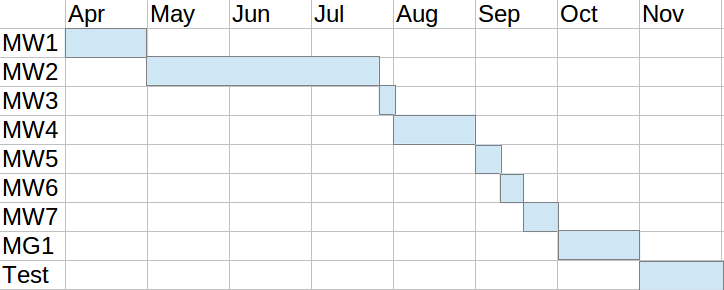
\includegraphics[width=3.in]{timetable.png}
%\caption{Timetable}
%\label{fig:plan}
%\end{figure}
